\section{Introduction}
徒手素描是人类历史上传达信息和表达情感的一种有效方式。素描草图不仅包含目标对象生动的分类特征,而且还包含抽象、多样的视觉表现。在本项目中,我们需要针对大小为 $28\times 28$ 的 25 类 草图图像(如图 \ref{fig:cate} 所示)构建深度学习模型以达到较好的分类效果,并对不同的网络结构性能进行比较。

\begin{figure}[ht]
    \centering
    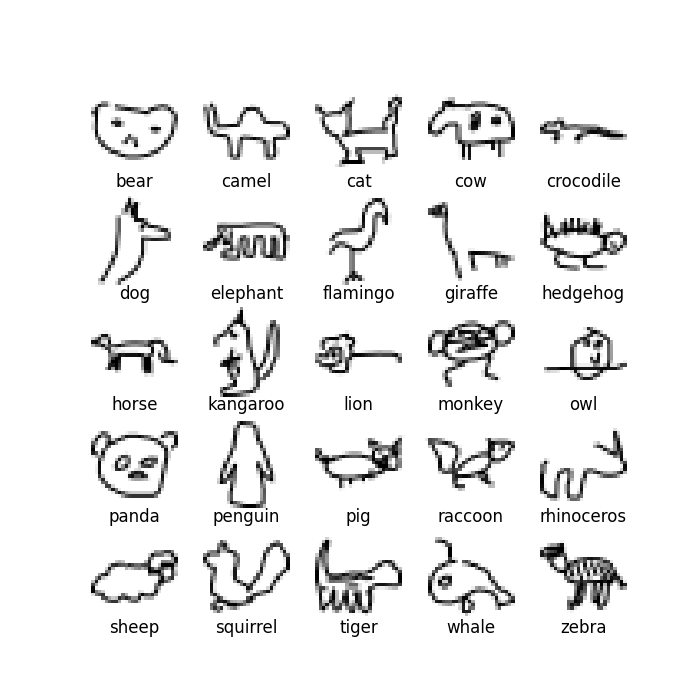
\includegraphics[width=7cm]{img/sketches.png}
    \caption{25个类别的草图}
    \label{fig:cate}
\end{figure}